%
% HCC用にIEEEフォーマットにしたもの
%
% 参考文献に適当なものを入れたい
%  Dynamic Queryとか no-click browsingが気持ちよい理由
%
%  https://dl.acm.org/doi/abs/10.1145/964696.964706 五十嵐氏の カスケーディングメニューのトラバース
%
% tree traverseという言葉を使いたい
%
% Dasher, LensBar
%
% Abstractが210語あるので減らす
%
\documentclass[conference]{IEEEtran}
\IEEEoverridecommandlockouts

\usepackage{cite}
% \usepackage{amsmath,amssymb,amsfontOBs}
% \usepackage{algorithmic}
\usepackage{graphicx}
% \usepackage{textcomp}
% \usepackage{xcolor}

\usepackage{here} % [H]とするとその場所に配置されるらしい
\long\def\comment#1{}

\long\def\comment#1{}

\long\def\ttt#1{\texttt{\textbf{\small #1}}}
\long\def\tsf#1{\textsf{\small{#1}}}
\long\def\tit#1{\textit{\small{#1}}}

\def\up{\tsf{▲}}
\def\down{\tsf{▼}}
\def\right{\tsf{▶}}
\def\left{\tsf{◀}}

\def\SC{Serencast}
\def\SB{Scrapbox}

\begin{document}

\title{No-click browsing of large hierarchical data}
%
% zero-click? no-click? clickless?
% zero-click searchとかclickless searchとかいうのは、Google検索の結果だけ見てクリックをしないことをそう呼ぶらしい
% no-click search という言葉も使われている
%

\author{\IEEEauthorblockN{Toshiyuki Masui}
  \IEEEauthorblockA{
    % \textit{Faculty of Environment and Information Studies}\\
    \textit{Keio University} \\
    % Fujisawa, Japan \\
    5322 Endo, Fujisawa, Kanagawa 252-0882, Japan \\
    masui@pitecan.com
  }
}

\IEEEoverridecommandlockouts
\IEEEpubid{\makebox[\columnwidth]{978-1-7281-6901-9/20/\$31.00~\copyright2020 IEEE\hfill} \hspace{\columnsep}\makebox[\columnwidth]{ }}

\maketitle

\IEEEpubidadjcol

\begin{abstract}
We introduce a novel simple interaction technique for finding and browsing
data in a large hierarchical database using only two keys.

Finding data from a huge hierarchical database takes time
because users should traverse the tree using a mouse or a keyboard,
and click a ``select'' button to check the content.
If the data was not appropriate,
they should go to the next entry and perform the selection task again.

In the past, when only a small number of ``channels'' were available
from broadcast TV stations, users could simply rotate
a television dial to select a channel and watch a program.
We introduce a simple interaction technique called ``\textit{Gear}'',
with which users can select an entry from a large hierarchical database and
browse it instantly, just like we could select a channel and enjoy a program
using old television dials.
\end{abstract}

\begin{IEEEkeywords}
  Input device, Information navigation, No-click browsing,
  Hierarchical data, Gear, Serencast
\end{IEEEkeywords}

% Input device, Information navigation, No-click browsing, Hierarchical data, Gear, Serencast

\section{Introduction}

% 大量のコンテンツから見たいものを捜して再生するのは大変である
% 
% 1. 階層から捜すのが大変
% 2. みつけたものをConfirmする手間がいる

Huge amount of movies, musics, and other programs are available on the web, but
finding and viewing a program is not easy because
(1) finding a program takes time, and
(2) a ``confirm'' operation (clicking something or typing a key)
is required for viewing the content.
%
The confirm operations was not required on old TVs and radios,
because we could enjoy TV/radio programs
as soon as we rotated a TV channel dial or a tuning dial of the radio.
%
It is always convenient to view the contents of the selected item
as soon as we find it.
We call such viewing style as ``\tit{no-click browsing}''.

We can perform no-click browsing on the ``column view'' mode of Finder.app on
MacOS using four keys.
In the column view mode, 
the contents of the file is shown at the right side of the window
as soon as we select a file in a folder (Figure \ref{noclickfinder}).
When we type an arrow key and select another file,
the contents is shown instantly without a confirm operation.

\begin{figure}[H]
  \centerline{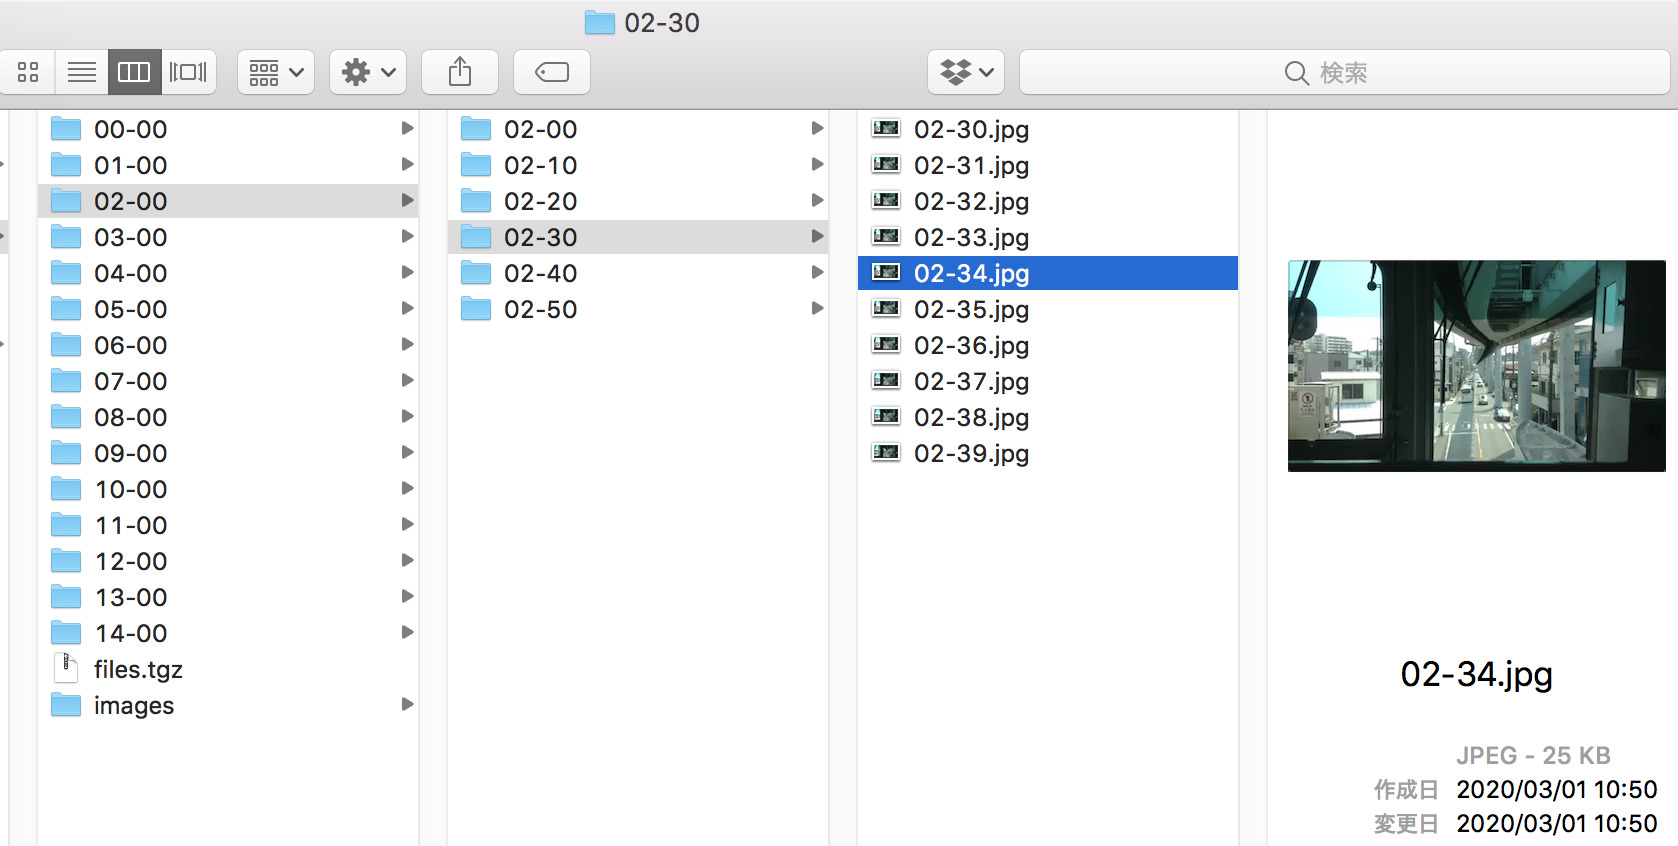
\includegraphics[width=70mm,bb=0 0 839 423]{figures/10d7ca6c55aa93ebcdab799246e4c087.jpg}}
  \caption{No-click browsing on the ``column view'' of Finder.app.}
  \label{noclickfinder}
\end{figure}

We could use no-click browsing on old TVs and radios because the number of
broadcast channels were limited.
Likewise, no-click browsing on Finder.app is useful
when the number of files in a folder is not very large.

No-click browsing is not popular on modern GUI of personal computers.
People are used to click-based browsing on web browsers and other
information visualization systems.
People can navigate through a huge information space by
clicking links, zooming and scrolling by dragging, and using other GUI techniques.
These techniques are useful for finding an item in a large information space,
but many clicks and drag operations are required,
and the contents of the items are usually not shown during the search.

It would be better
if we could perform the navigation task using devices that have only two keys.
%
We have developed a new navigation technique called ``\tit{Gear}'' for no-click browsing,
where users can explore a large hierarchical database by using only two keys.


\section{Navigation method of Gear}
\label{navigation}

Interaction with Gear is based on the following simple principles.
Two operations,
{\up} (up) and {\down} (down), are used for the navigation.

\begin{enumerate}
\item A portion of hierarchical data is shown to the user.

\item One element in the list is selected and highlighted.

% \item Display the selected element, its siblings, its ancestors and their siblings.

\item When an element is selected, its siblings, its ancestors and their siblings are displayed
around the selected element.

\item Users can issue {\up} to select the element above the currently selected element,
or issue {\down} to select the element below the selected element.
Whenever the selection is changed, 3) is performed.
If the depth of the newly selected element is different from the currently
selected element, siblings of the currently selected element disappear.

\item When a newly selected element has children and the user performs no further action,
the first child of the selected element is newly selected, and 3) is performed.
As a result, all the siblings of the newly selected element
(the first child of the currently selected element) appear in the list.

\end{enumerate}

We show how Gear works, using a hierarchical data structure of
a shop list in a shopping mall shown in Figure \ref{fig1} as example data.
A rectangles with a thick border represents a shop category, and
other rectangles represent individual shops.

\begin{figure}[H]
  \centerline{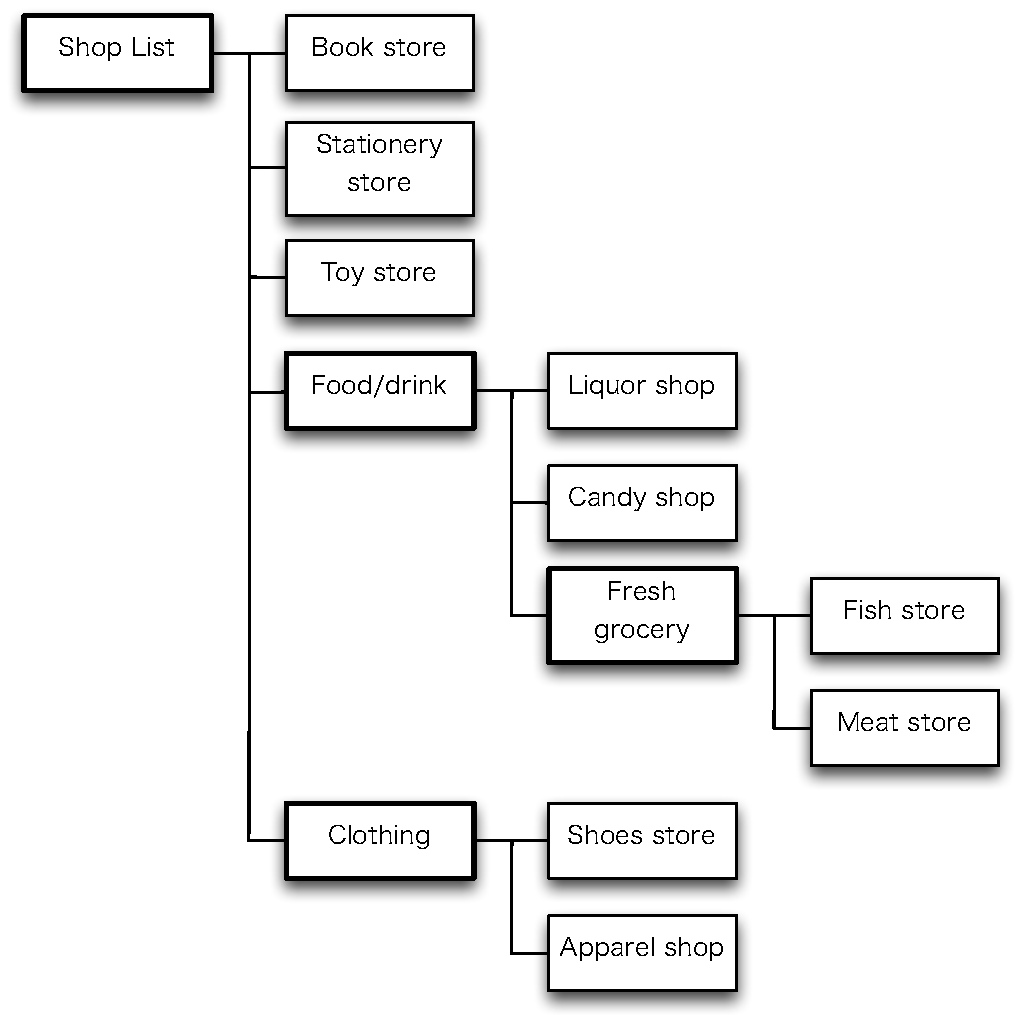
\includegraphics[width=70mm,bb=0 0 490 490]{figures/fig1.pdf}}
  \caption{Sample data: shop list in a shopping mall.}
  \label{fig1}
\end{figure}

When a user starts the exploration, only the shops and categories
at the top level are displayed (Figure \ref{fig2}).
When the user issues {\down},
the second element (\tsf{Stationery store}) is selected (Figure \ref{fig3}).

\def\menuwidth{22mm}

\begin{figure}[H]
  \begin{minipage}{0.45\hsize}
    \centerline{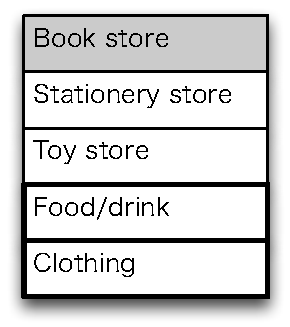
\includegraphics[width=17mm, bb=0 0 139 157]{figures/fig2.pdf}}
    \caption{Initial display.}
    \label{fig2}
  \end{minipage}
  \begin{minipage}{0.45\hsize}
    \centerline{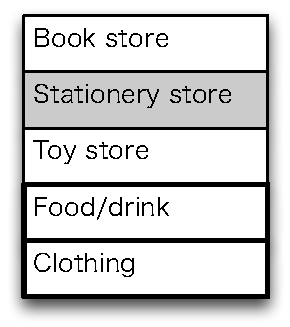
\includegraphics[width=17mm,bb=0 0 139 157]{figures/fig3.pdf}}
    \caption{Typing {\down}.}
    \label{fig3}
  \end{minipage}
\end{figure}

If the user issues {\down} two more times, 
\tsf{Food/drink} category is selected (Figure \ref{fig4}).
If the user stops the operation and waits for a moment, the shops under the \tsf{Food/drink}
category are automatically displayed,
and the first entry (\tsf{Liquor shop}) is selected (Figure \ref{fig5}).

\begin{figure}[H]
  \begin{minipage}{0.45\hsize}
    \centerline{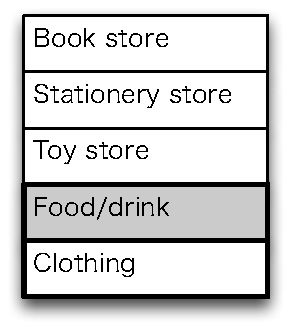
\includegraphics[width=17mm,bb=0 0 139 157]{figures/fig4.pdf}}
    \caption{Selecting Food/drink.}
    \label{fig4}
  \end{minipage}
  \begin{minipage}{0.45\hsize}
    \centerline{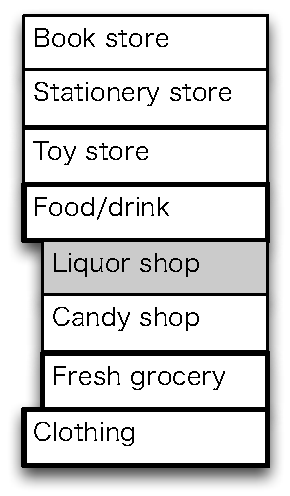
\includegraphics[width=17mm,bb=0 0 139 238]{figures/fig5.pdf}}
    \caption{Selecting Liquor shop.}
    \label{fig5}
  \end{minipage}
\end{figure}

When the user issues {\down} twice here,
\tsf{Fresh grocery} category is selected (Figure \ref{fig6}).
%
If the user keeps issuing {\down}, 
the list will change to Figure \ref{fig8},
without expanding the children of \tsf{Fresh grocery}.

\begin{figure}[H]
  \begin{minipage}{0.45\hsize}
    \centerline{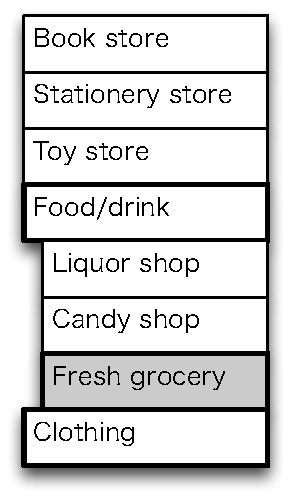
\includegraphics[width=17mm,bb=0 0 139 238]{figures/fig6.pdf}}
    \caption{Selecting Fresh grocery.}
    \label{fig6}
  \end{minipage}
  \begin{minipage}{0.45\hsize}
    \centerline{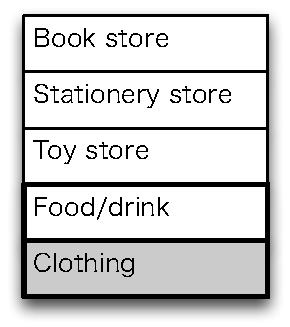
\includegraphics[width=17mm,bb=0 0 139 157]{figures/fig8.pdf}}
    \caption{Selecting Clothing.}
    \label{fig8}
  \end{minipage}
\end{figure}

If the use stops issuing {\down} at Figure \ref{fig6},
the shops under category \tsf{Fresh grocery} is automatically selected (Figure \ref{fig7}).
%
When the user issues {\up} here, \tsf{Fresh grocery} is selected,
and the shops under \tsf{Fresh grocery} disappears, 
resulting in the same state as Figure \ref{fig6}.
If the user issues {\up} two more times, the display changes to the state
shown in Figure \ref{fig5},
and one more {\up} will set the system to the state of Figure \ref{fig4}.

If the user issues {\down} in Figure \ref{fig4}, the next visible entry
(\tsf{Clothing}) is selected (Figure \ref{fig8}), and the state changes to Figure \ref{fig9}.

\begin{figure}[H]
  \begin{minipage}{0.45\hsize}
    \centerline{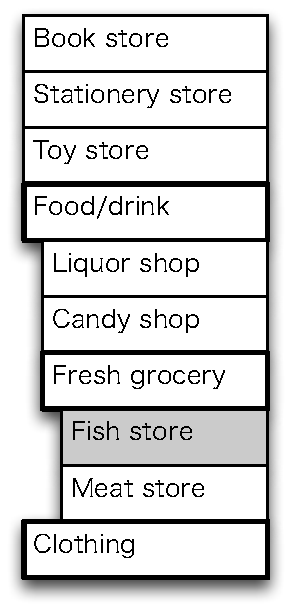
\includegraphics[width=17mm,bb=0 0 139 292]{figures/fig7.pdf}}
    \caption{Selecting Fish store.}
    \label{fig7}
  \end{minipage}
  \begin{minipage}{0.45\hsize}
    \centerline{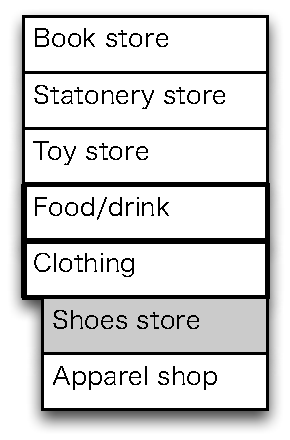
\includegraphics[width=17mm,bb=0 0 139 211]{figures/fig9.pdf}}
    \caption{Selecting Shoes store.}
    \label{fig9}
  \end{minipage}
\end{figure}

When the user issues {\down} twice in Figure \ref{fig7},
\tsf{Clothing} is selected, and the category under \tsf{Food/drink} will shrink (Figure \ref{fig8}).

In this way, users can explore the hierarchical structure
only by issuing {\up} and {\down} at the right timing.

\section{Serencast: a no-click browsing service}

To prove that Gear is useful for selecting an entry from a
large hierarchical database,
we developed the ``\tsf{\SC}'' service\footnote{
  \tsf{https://Serencast.com/}
}, where users can enjoy movies, musics, and other web services
on the browser with the Gear interface without clicking an entry.
{\SC} is implemented in JavaScript and runs on modern web browsers.
%
{\SC} uses the ``\tsf{\SB}'' wiki service\footnote{
  \tsf{https://Scrapbox.io/}
} for listing the contents of the hierarchical database.
{\SB} is an interactive wiki
system where users can share and edit texts on the web browser,
just like the Google Docs system.

When we list the URLs of Web pages of
movies and musics on a {\SB} page,
we can use {\SC} service
for using the Gear interface to select a program from the
list on {\SB} pages and automatically play it on the browser.

Figure \ref{movielist} shows the movie list defined in a {\SB} page.

\comment{
\begin{figure}[H]
  \centerline{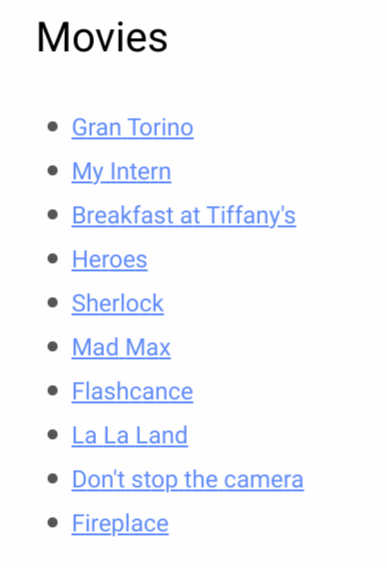
\includegraphics[width=30mm,bb=0 0 387 568]{figures/2b97930bf5730fcaf4d9c0adeb9c5f6e.png}}
  \caption{A movie list page on {\SB}.}
  \label{movielist}
\end{figure}
}


\begin{figure}[H]
{\scriptsize
\begin{verbatim}
Movies and videos
 [https://www.netflix.com/watch/70105600 Gran Torino]
 [https://www.netflix.com/watch/80047616 My Intern]
 [https://www.netflix.com/watch/330201 Breakfast at Tiffany's]
 [https://www.netflix.com/watch/70080178 Heroes]
 [https://www.netflix.com/watch/70174781 Sherlock]
 [https://www.happyon.jp/watch/100048550 Mad Max]
 [https://www.netflix.com/watch/60010351 Flashdance]
 [https://www.netflix.com/watch/80095365 La La Land]
 [https://www.netflix.com/watch/81191988 Don't stop the camera]
 [https://youtube.com/embed/AtZr9g2vwrI?autoplay=1 Fireplace]
\end{verbatim}
}
\caption{A movie list page on {\SB}.}
\label{movielist}
\end{figure}

When we access this {\SB} page from {\SC},
``Gran Trino'' from Netflix automatically starts in the right side of the screen,
just like a TV program starts when we rotate the channel dial of an old television.
When the user pushes the {\down} key twice,
``Breakfast at Tiffarny's'' is selected and
the movie starts automatically at the right side of the screen (Figure \ref{tiffany}).

\begin{figure}[H]
  \centerline{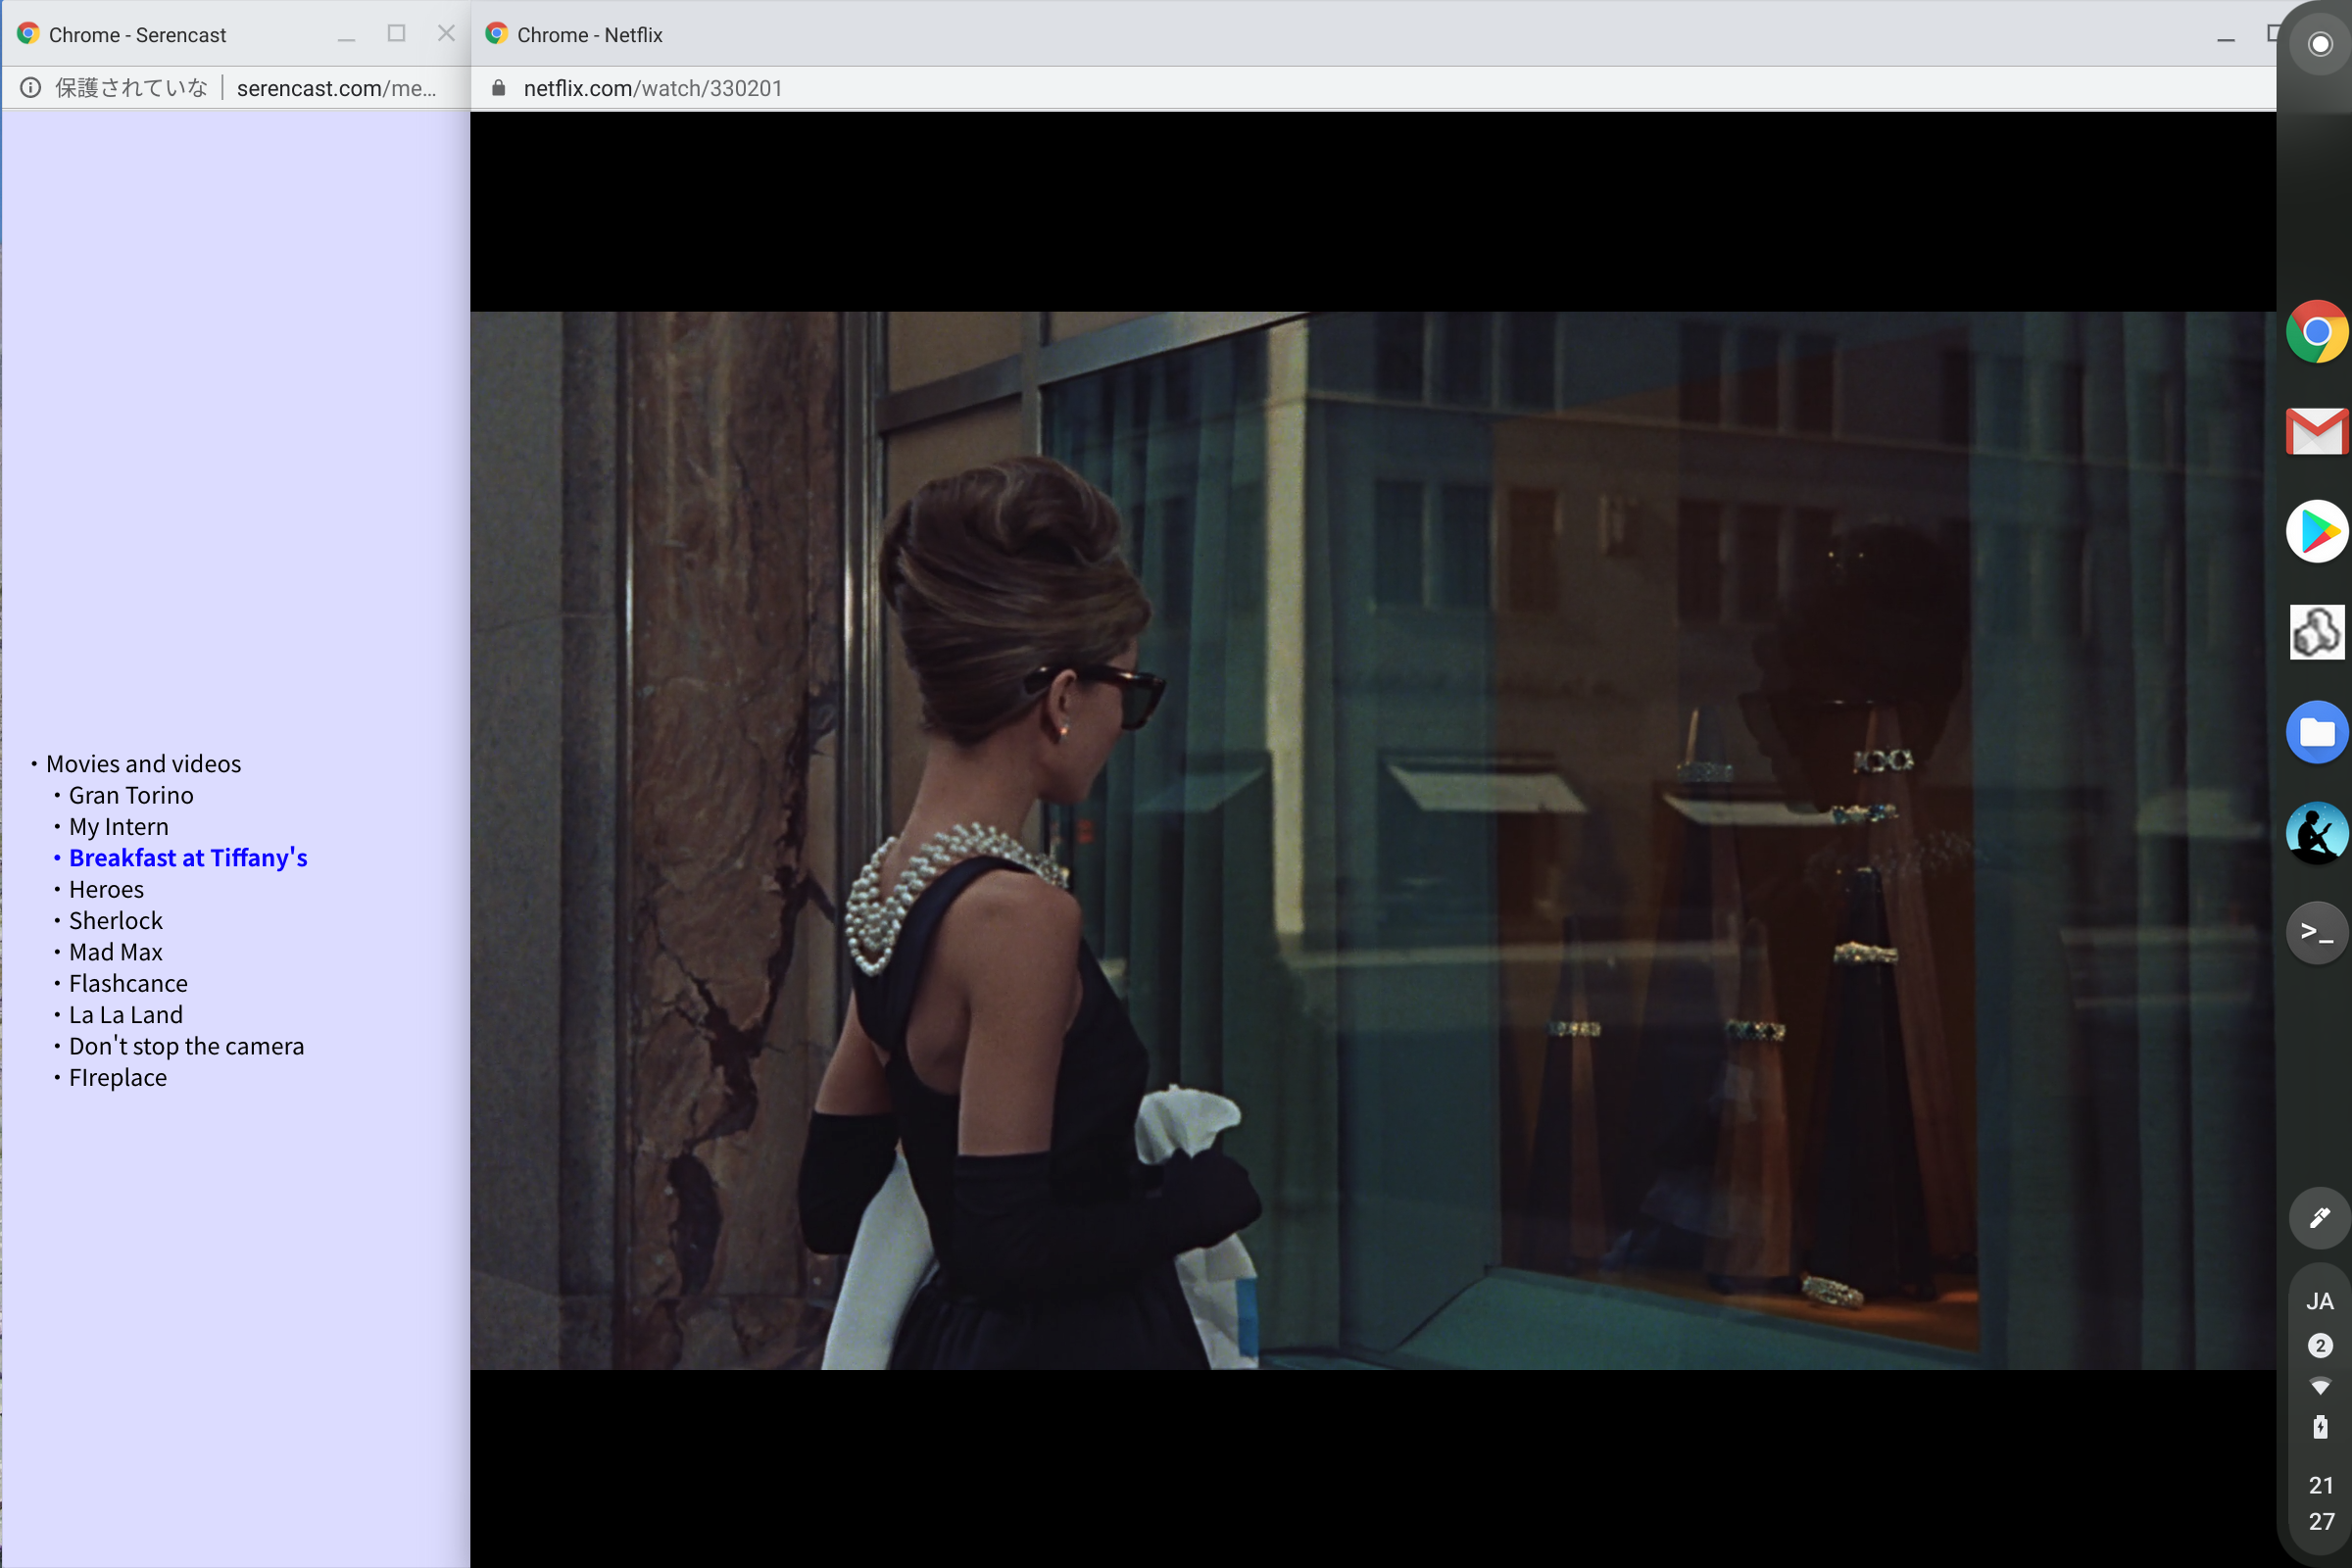
\includegraphics[width=65mm,bb=0 0 2400 1600]{figures/e8ae562a5a68a1955ac70b4faed9a146.png}}
  \caption{Watching ``Breakfast at Tiffany's'' on Serencast.}
  \label{tiffany}
\end{figure}


In the above example, we can select only one of the 10 movies from the movie list.
But we can add more data by hierarchically providing contents in {\SB} pages.

Since anybody can edit {\SB} pages and construct the hierarchical data,
people can enjoy creating their own database by editing their {\SB} pages.
When someone wants to advertise their works,
he can create his {\SB} pages
and give them to other people so that they can watch the pages.

\section{Discussion}

\subsection{Input devices for Gear}

Since only two switches are required in the Gear interface,
almost any kind of input devices can be used for Gear.
We have tried various input devices and collected experiences.

\subsubsection{Keys and buttons}

The simplest input device for Gear may be keyboards and push buttons.
Gear works pretty comfortably with arrow keys on a PC.
Various HID devices\footnote{
  \tsf{https://en.wikipedia.org/wiki/Human\_interface\_device}
} are available on the market, and
all such devices can be used as input devices for Gear.

\subsubsection{2-way lever}

We have also tried to use a paddle-like device for generating {\up} and {\down} (Figure \ref{paddle}).
Users can push the puddle to the right to generate {\up} and
left to generate {\down}.
Pressure sensors are installed on the puddle, and
many {\up}'s are generated when the user pushes the puddle strongly.

\begin{figure}[H]
  \begin{minipage}{0.49\hsize}
    \centerline{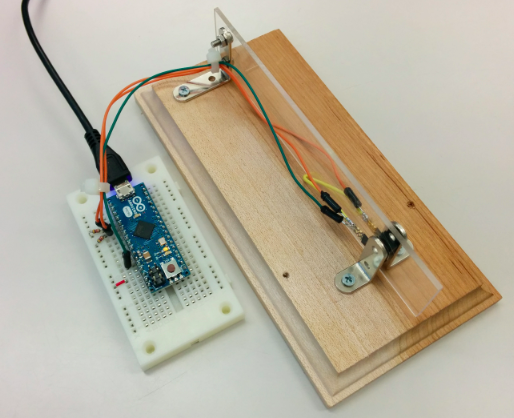
\includegraphics[width=38mm,bb=0 0 514 418]{figures/3c2de63899653056f3c6be835b9aaf43.png}}
    \caption{Paddle device for Gear.}
    \label{paddle}
  \end{minipage}
  \begin{minipage}{0.49\hsize}
    \centerline{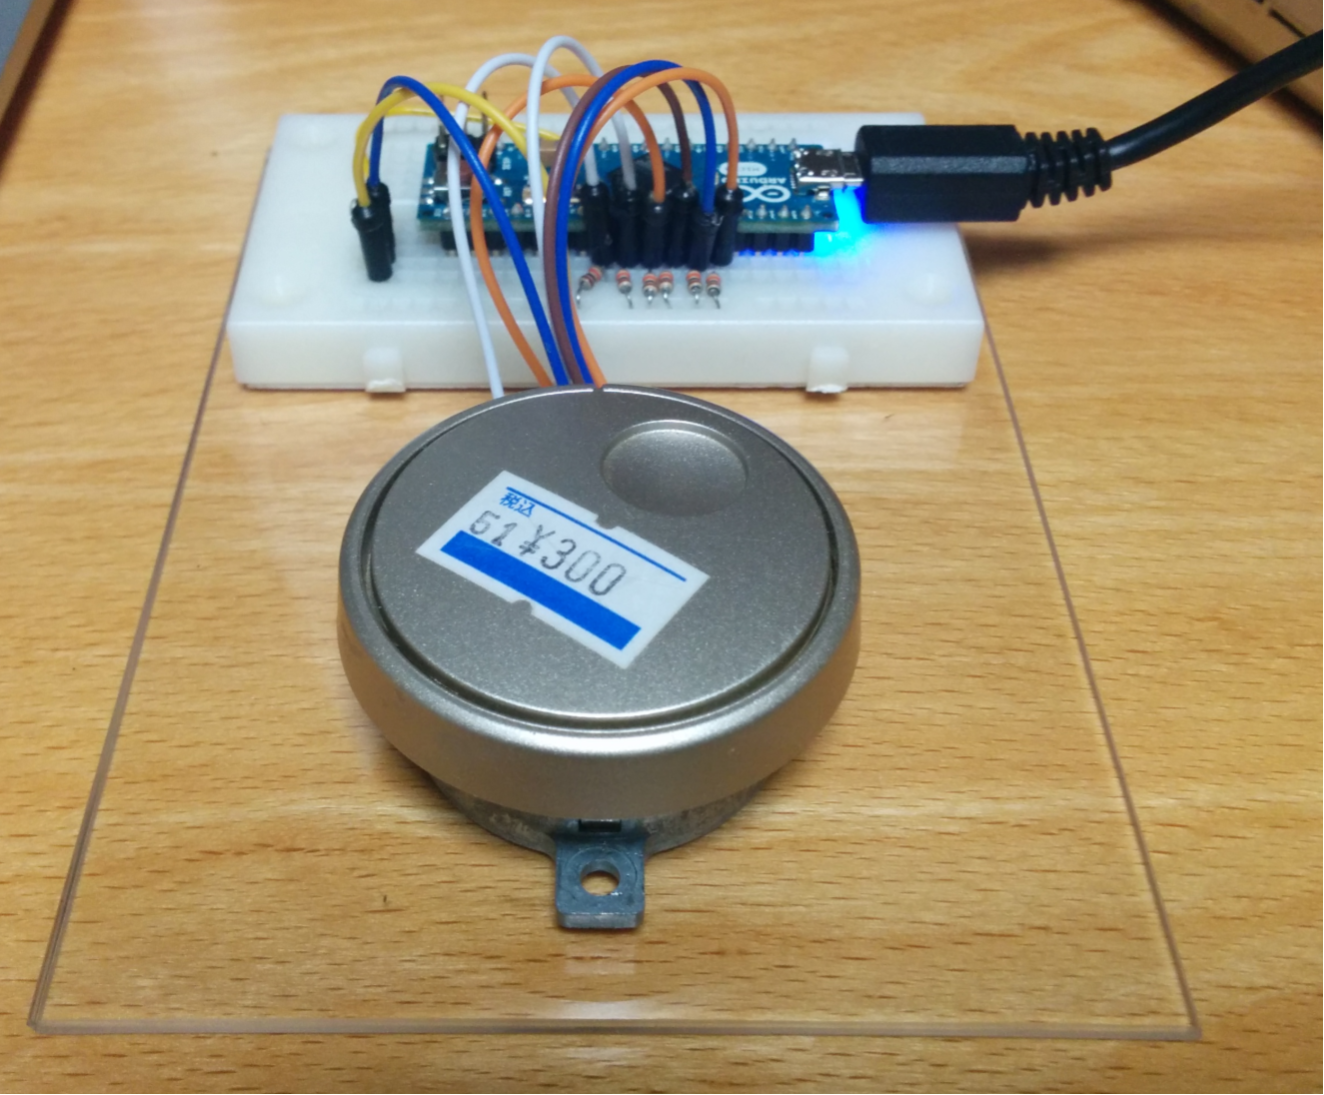
\includegraphics[width=38mm,bb=0 0 1324 1095]{figures/7a2c685b930cd30a267f4d564a8079be.png}}
    \caption{Using a jog dial.}
    \label{jog}
  \end{minipage}
\end{figure}

Controlling the speed of the scrolling of Gear by pressure is convenient,
since sometimes users want to jump to an entry far from current position.
That behavior is similar to the key-repeat feature of computer keyboards.

\subsubsection{Rotating devices}

We then tried various rotating devices for Gear.
%
We tried mouse wheels first, and found that they are very suitable for Gear,
because we are good at controlling our finger with precision.

Many kinds of rotating input devices have been used for controlling TVs and VCRs so far.
For example, ``jog dials'' have been widely used for controlling VCRs,
and we tried the device for Gear (Figure \ref{jog}).

\begin{figure}[H]
  \begin{minipage}{0.49\hsize}
    \centerline{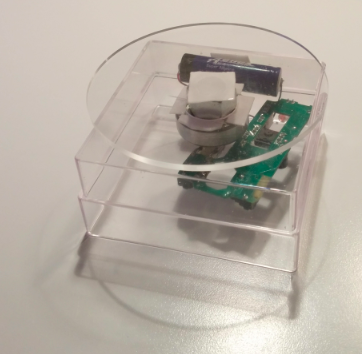
\includegraphics[width=38mm,bb=0 0 362 354]{figures/ff2d18e66f9a4655dbb5e22e0bb9a0ae.png}}
    \caption{A disk-based device for Gear.}
    \label{disk}
  \end{minipage}
  \begin{minipage}{0.49\hsize}
    \centerline{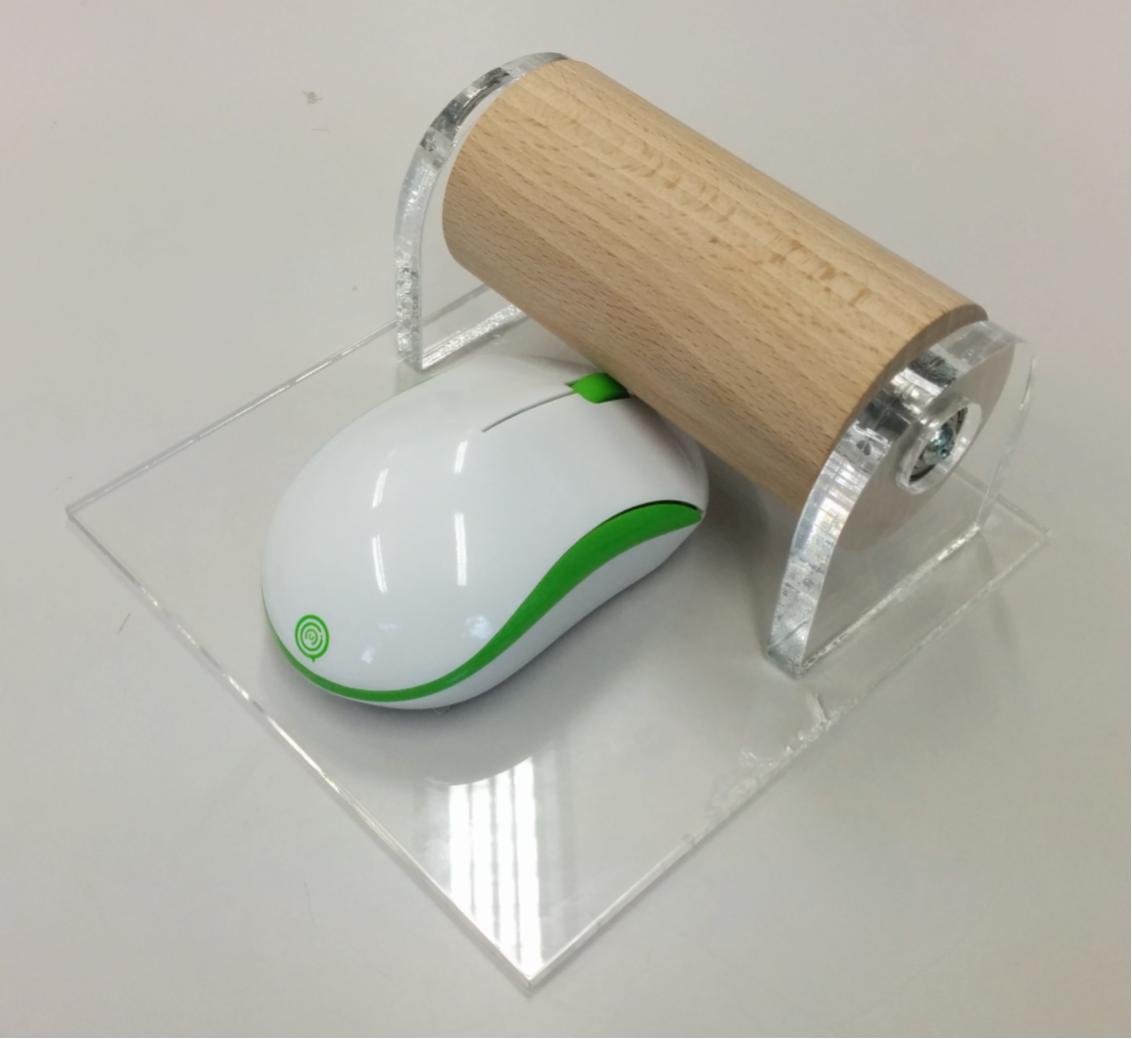
\includegraphics[width=38mm,bb=0 0 1132 1039]{figures/6ff91502ea4f3f3c47840c887148ada9.png}}
    \caption{Using a roller.}
    \label{roller}
  \end{minipage}
\end{figure}

We have also tried using a cylinder for Gear.
The rotating cylinder shown in Figure \ref{roller} is touching the mouse wheel, and
mouse wheel events are generated as the user rotates the cylinder using his arm or hand.

After trying these devices, we found that controlling rotating devices
like jog dials and cylinders are not as easy as we expected,
because precise control of an arm or a hand is fairly difficult.
People are good at controlling fingers, but people are usually not very good at
controlling arms and hands precisely.

After trying various devices, it became clear that simple buttons or
wheels can be put at anywhere like on the table or under a chair, and
we felt that the integration of furniture and input devices will be
important in the IoT age\cite{10.1145/2494091.2497326}.
%
If we can install the devices neatly on furniture and beds,
people with disabilities can easily use them.

\subsection{Comparison with existing navigation methods}

To compare the speed of Gear with conventional navigation method,
we created two applications for checking how fast a user can select an entry
from a large hierarchical database.
%
Both applications behaves the same way:
a user can set the date to a specific time to see a photo in a 15-minute monorail trip.
%
Using the first one (App1), a user can set the time using Gear
with up/down arrow keys for {\up} and {\down} (Figure \ref{monorailgear}).

Using the second one, a user can set the time using the \ttt{{\textless}input type="time"{\textgreater}} tag of HTML (Figure \ref{monorailinput}).
Users can first set the value of the ``minute'' value at the top-left using up/down cursor keys,
and move to the right with the right-arrow key and set the ``second'' value with up/down arrow keys.

\begin{figure}[H]
  \begin{minipage}{0.49\hsize}
    \centerline{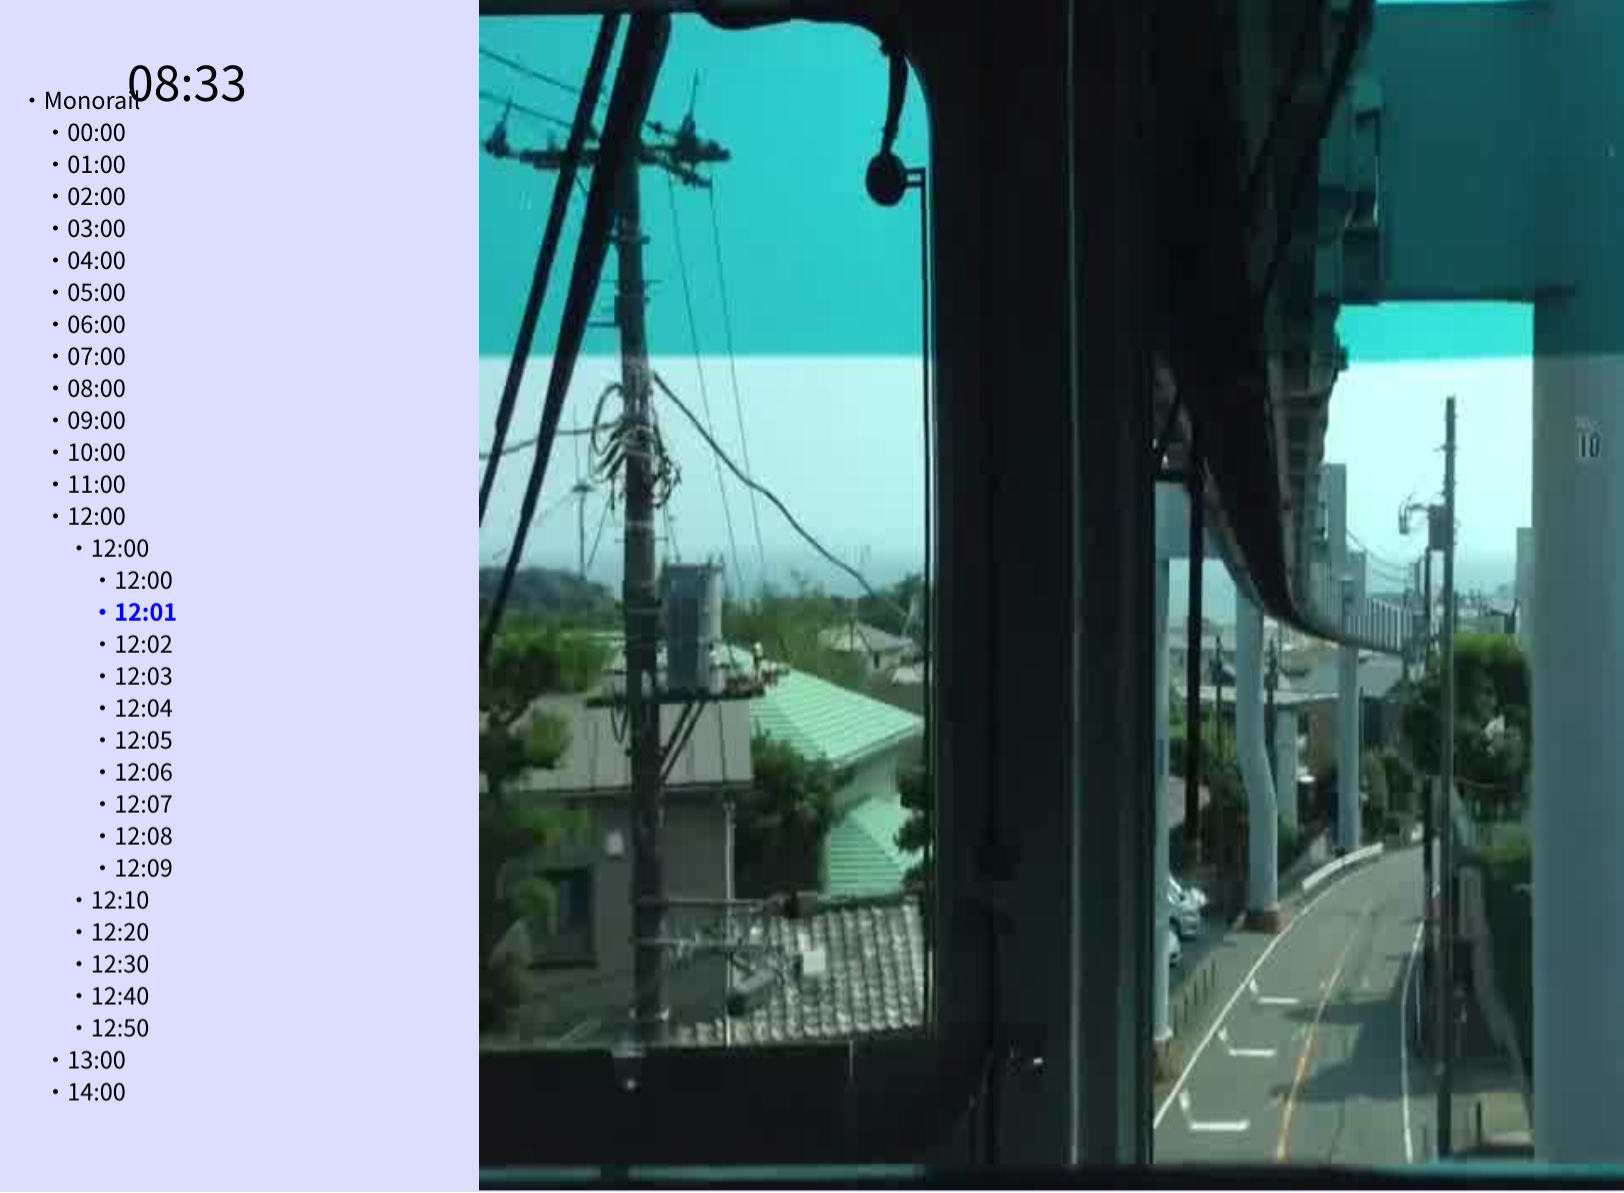
\includegraphics[width=40mm,bb=0 0 1624 1193]{figures/75007628f75ef1038bd5737e10a728b7.png}}
    \caption{App1: Gear-based application for finding a monorail picture.}
    \label{monorailgear}
  \end{minipage}
  \begin{minipage}{0.49\hsize}
    \centerline{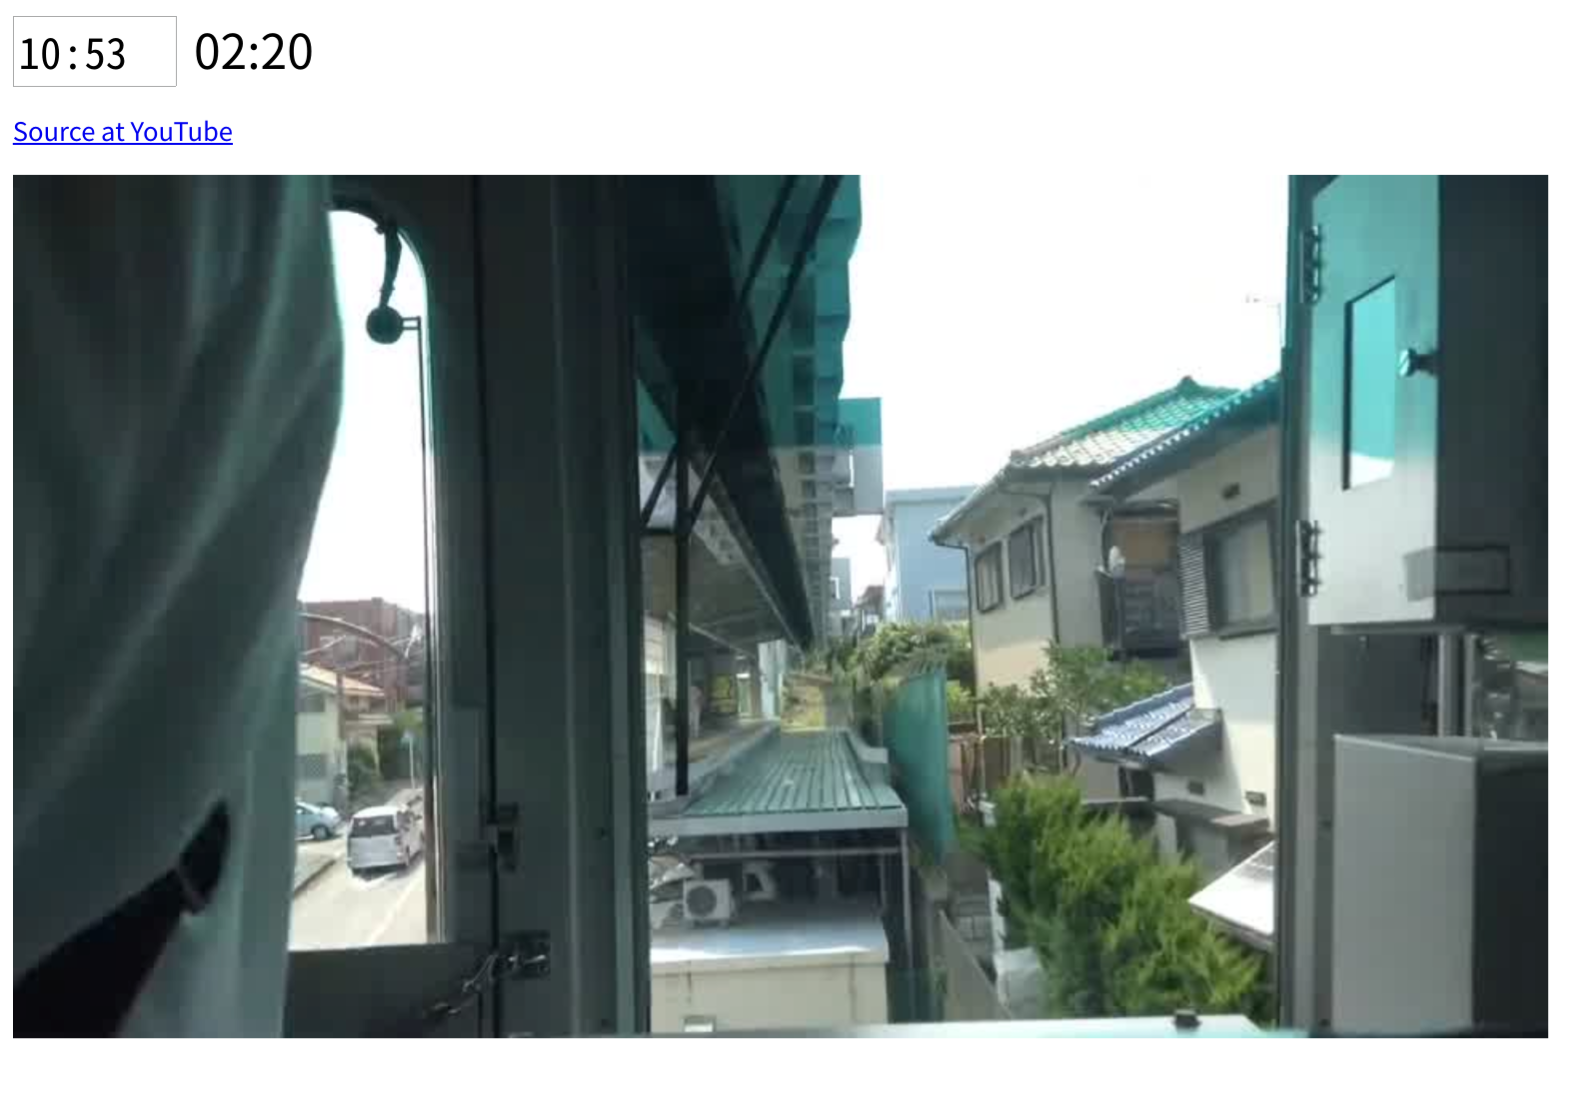
\includegraphics[width=40mm,bb=0 0 1596 1116]{figures/325208a6d94c68e4f08e61a67df419c4.png}}
    \caption{App2: using input element.}
    \label{monorailinput}
  \end{minipage}
\end{figure}

On both applications, a random target time is displayed on the screen and the subjects are
asked to set the time to the displayed target time.
After repeating the task 5 times, the average time is shown to the user, and the value
was reported.

We asked 5 people to try these tasks 10 times, and the result of the experiment is
shown in Figure \ref{monorailtime}.

\begin{figure}[H]
\centerline{
  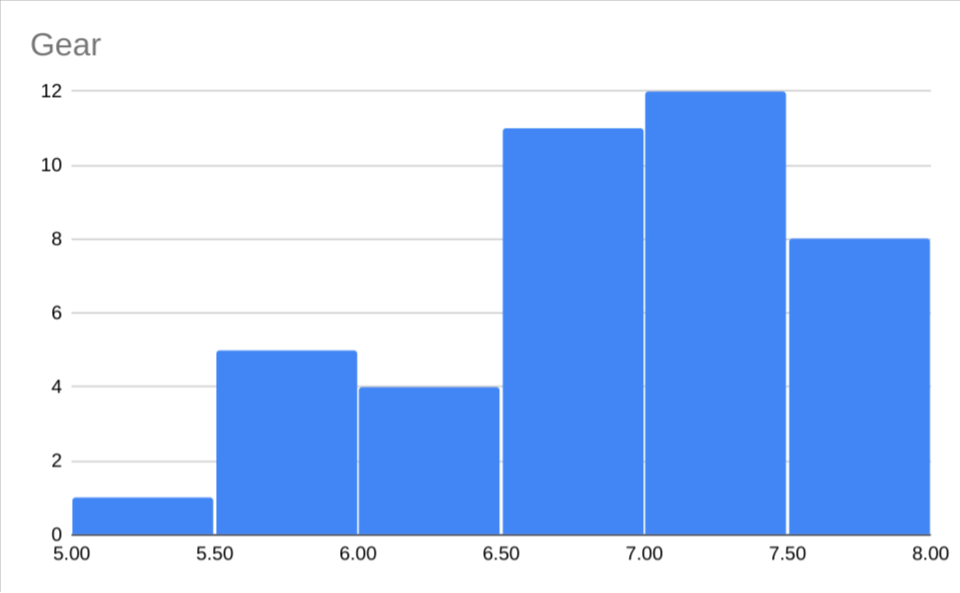
\includegraphics[width=43mm,bb=0 0 960 593]{figures/6c39f199b341e30ffc28850afbd90a5a.png}
  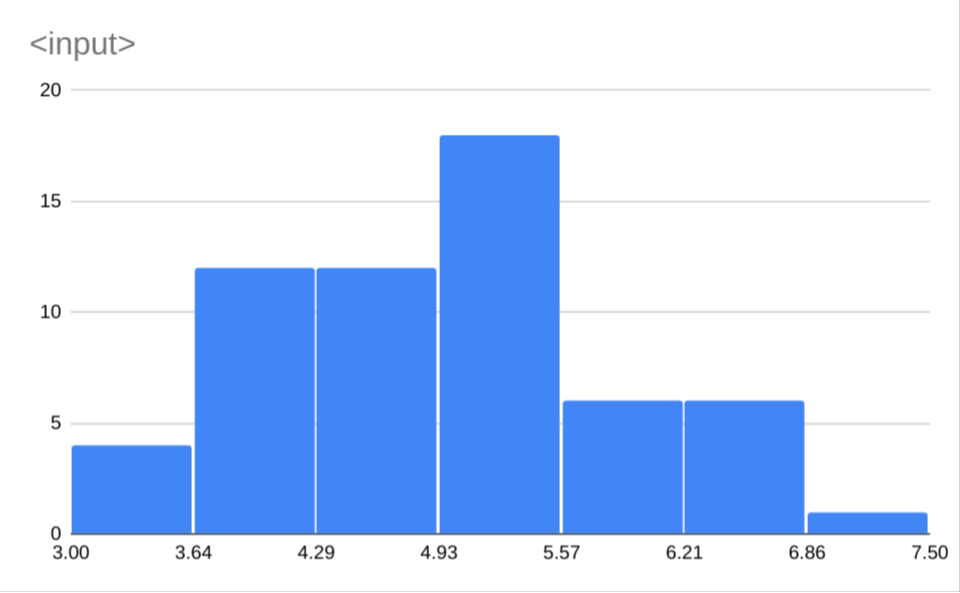
\includegraphics[width=43mm,bb=0 0 960 593]{figures/de3f0545e0d0d8dfb9708d2420fb5407.png}
}
\caption{Average search time of App1 and App2.}
\label{monorailtime}
\end{figure}

The average time for finding an entry using Gear was 6.84s,
and the average time using standard \ttt{{\textless}input{\textgreater}} was 4.96s.
It takes about 40\% longer than using conventional method.
The standard deviations were 0.71s and 0.93s, respectively.
%
This is a little bit disappointing,
but we are happy to see that
no-click browsing with Gear is not too slower than
conventional methods using four keys.
%
We have also tried using Finder.app for the same data (Figure \ref{noclickfinder}), and
got similar results.

Using a conventional hierarchical menu,
child elements are displayed automatically when their parent element is selected by a mouse.
The behavior is well understood by computer users,
and Gear's automatic transition (e.g. from Figure \ref{fig4} to Figure \ref{fig5})
looks familiar to users.

\subsection{Comparison with InfoVis techniques}

Various information visualization techniques like
Treemap\cite{Johnson:1991:TSA:949607.949654},
Hyperbolic Tree\cite{Lamping:1995:FTB:223904.223956},
and Sunburst\cite{Stasko:2000:FDN:857190.857683}
have been proposed for visualizing large hierarchical data.
Zooming user interface (ZUI) systems like
Pad\cite{Perlin:1993:PAA:166117.166125} and
Pad++\cite{Bederson:1994:PZG:192426.192435}
can also be used for handling large hierarchical data laid out in a 2D space.
%
These visualization techniques and descendent technologies have become popular these days and
all of these systems are useful for understanding the structure of
large hierarchical data.
However, users of these systems have to use a pointing device
to take full advantage of these methods, and
no-click browsing is not supported.

It seems to be a good idea to use Gear on more conventional visualization techniques like
TreeView\footnote{
  \textsf{http://en.wikipedia.org/wiki/Tree\_view}
}, where four keys are used for navigation.
%
We can also use Gear on a 1D zooming system like
LensBar\cite{Masui:1998:LVB:647341.721215},
where pointing devices are mainly used for navigation.

% is also a ZUI system for handling large hierarchical data,
% but the same data structure used in LensBar can be used for Gear.
% Users can use a pointing devices when it is appropriate,
% and use two keys or a disk device when pointing devices is not available.

\subsection{Using Gear in the wild}

The author have been using Gear in his living room for several years
with a small personal computer connected to a 60-inch TV monitor.
The database is managed on {\SB}, and
a mouse wheel of a wireless Bluetooth mouse is used for Gear interface.
With Gear, the user can enjoy all available contents on the web with the mouse wheel
without selecting the source of the movies, animes, and musics from Amazon, Netflix, etc.

We can enjoy using Gear everywhere using a stick PC and a wireless mouse,
just like Amazon FireTV can be used for the same purpose.
Using {\SC} is more fun for the author, since no-click browsing is more comfortable than
selection-based interface on existing systems.

We demonstrated Gear at an exhibition
and asked more than 100 people to try it
(Figure \ref{exhibition}).
%
Since the only thing a user could do with the Gear device was to rotate a wheel,
users seemed to be able to understand the behavior of Gear with trials and errors.
% 
% a user can use the device and see what happens without thinking about
% other interactions.
% 
Although using only one rotating device for navigation was a new experience for the visitors,
they seemed to have felt it natural in a short while.

\begin{figure}[H]
\centerline{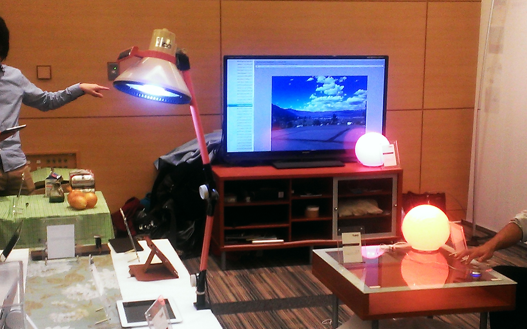
\includegraphics[width=60mm,bb=0 0 527 329]{figures/c520d5dfbd06c532d48d324a7019b00c.png}}
\caption{People at the right using a wheel device at an exhibition.}
\label{exhibition}
\end{figure}

% Selecting a content only by rotating a dial is very 気持ち良い。
% 音楽ソース、ニュースソース、動画、Wikipediaなどあらゆるものをダイヤルやペダルだけで検索できる

\section{Conclusion}

We have developed a new simple interaction method ``Gear'' for exploring
a large hierarchical data structure.
A Gear user can easily find an entry in a huge hierarchical database
only by using two keys or a rotating device that can be installed at
wide ranges of locations where conventional devices do not fit.
We are hoping to install various implementations of Gear and try them at
various places like kitchens, restrooms, etc.

\small{
\bibliographystyle{IEEEtran}
\bibliography{paper}
}

\end{document}

